%
%  THESISBOEK
%
%  Dit bestand zorgt voor algemene (layout)definities, en groepeert de
%  afzonderlijke LaTeX-files tot een geheel.
%
%  @author Erwin Six, David De Reu, Brecht Vermeulen
%

\documentclass[11pt,a4paper,oneside,notitlepage]{book}
\usepackage[english]{babel}
\usepackage{algorithmic}
\usepackage{algorithm}
\usepackage{amsthm}
\usepackage{hyperref}
\usepackage{array}
%\usepackage[nottoc]{tocbibind} % Bibliografie in ToC; zie tocbibind.dvi

% marges aanpassen
% (opmerking: moet *voor* inclusie van fancyhdr package komen)
\setlength{\hoffset}{-1in}
\setlength{\voffset}{-1in}
\setlength{\topmargin}{2cm}
\setlength{\headheight}{0.5cm}
\setlength{\headsep}{1cm}
\setlength{\oddsidemargin}{3.5cm}
\setlength{\evensidemargin}{3.5cm}
\setlength{\textwidth}{16cm}
\setlength{\textheight}{23.3cm}
\setlength{\footskip}{1.5cm}

\usepackage{fancyhdr}
\usepackage{graphicx}
% \usepackage[colorlinks]{hyperref}
% Het bibliografisch opmaak bestand.
\bibliographystyle{unsrt}
%\bibliographystyle{bibliodutch}
%\bibpunct{[}{]}{,}{n}{,}{,}

\newtheorem{mydef}{Definition}
\newtheorem{foundation}{Foundation}

\pagestyle{fancy}

\renewcommand{\chaptermark}[1]{\markright{\MakeUppercase{#1}}}
\renewcommand{\sectionmark}[1]{\markright{\thesection~#1}}

\newcommand{\headerfmt}[1]{\textsl{\textsf{#1}}}
\newcommand{\headerfmtpage}[1]{\textsf{#1}}

\fancyhf{}
\fancyhead[LE,RO]{\headerfmtpage{\thepage}}
\fancyhead[LO]{\headerfmt{\rightmark}}
\fancyhead[RE]{\headerfmt{\leftmark}}
\renewcommand{\headrulewidth}{0.5pt}
\renewcommand{\footrulewidth}{0pt}

\fancypagestyle{plain}{ % eerste bladzijde van een hoofdstuk
  \fancyhf{}
  \fancyhead[LE,RO]{\headerfmtpage{\thepage}}
  \fancyhead[LO]{\headerfmt{\rightmark}}
  \fancyhead[RE]{\headerfmt{\leftmark}}
  \renewcommand{\headrulewidth}{0.5pt}
  \renewcommand{\footrulewidth}{0pt}
}

% anderhalve interlinie (opm: titelblad gaat uit van 1.5)
\renewcommand{\baselinestretch}{1.5}

% indien LaTeX niet goed splitst, neem je woord hierin op, of evt om splitsen 
% te voorkomen
\hyphenation{ditmagnooitgesplitstworden dit-woord-splitst-hier}

\begin{document}

%!!!!!!!!!!!!!!!!!!!!!!!!!!!!!!!!!!!!!!!!!!!!!!!!!!!!!!!!!!!!!!!!!!!!!!!!!!!!!!!!!!!!!!!!!!!!!!!!!
%!!!!!!!!!!!              onderaan/bovenaan elk blad thesistitel zetten                !!!!!!!!!!!
%!!!!!!!!!!!!!!!!!!!!!!!!!!!!!!!!!!!!!!!!!!!!!!!!!!!!!!!!!!!!!!!!!!!!!!!!!!!!!!!!!!!!!!!!!!!!!!!!!

% overzicht/samenvatting
%%  Overzichtsbladzijde met samenvatting

\newpage

{
\setlength{\baselineskip}{32pt}
\setlength{\parindent}{0pt}
\setlength{\parskip}{18pt}

\begin{center}

\noindent \textbf{\huge
Identifying experts through }
\textbf{\huge a framework for knowledge extraction}
\textbf{\huge from public online sources}

\setlength{\baselineskip}{12pt}
\setlength{\parindent}{0pt}
\setlength{\parskip}{12pt}

door 

Simon Buelens, Mattias Putman

Promotors: Prof.~Dr.~Ir.~Filip~De~Turck,~Elena~Tsiporkova~(Sirris),~Tom~Tourw\'{e}~(Sirris)\\
Scriptiebegeleiders: Anna~Hristoskova,~Tim~Wauters\\

Masterproef ingediend tot het behalen van de academische graad van\\
Master in de ingenieurswetenschappen: computerwetenschappen

Academiejaar 2010-2011\\
Faculteit Ingenieurswetenschappen\\
Voorzitter: Prof. Dr. Ir. Dani\"{e}l De Zutter\\
Vakgroep Informatietechnologie\\

\end{center}

\setlength{\baselineskip}{10pt}
\setlength{\parindent}{0pt}
\setlength{\parskip}{10pt}

\renewcommand{\baselinestretch}{1.1} 	% De interlinie afstand wat vergroten.
\small\normalsize                       % Nodig om de baselinestretch goed te krijgen.

\section*{Samenvatting}

Onderzoekers verliezen veel tijd met de zoektocht naar informatie gerelateerd aan hun onderzoeksdomein. Er bestaan bijna geen diensten die toelaten om aan de hand van trefwoorden een overzicht te verkrijgen met experts voor de opgegeven domeinen. Er is onderzoek naar disambiguatie van auteurs, maar deze worden meestal niet in combinatie gebracht met het opzoeken van experten, maar het indelen van publicaties (alhoewel de twee gerelateerd zijn).

In deze masterproef onderzoeken we de mogelijkheid om een framework op te stellen dat dit toelaat door online informatie op te zoeken, deze informatie in relatie te brengen met de correcte auteurs en gebruikers toe te laten dit framework te gebruiken om hierin te zoeken. De nadruk van het framework ligt op de disambiguatie van auteurs (aan de hand van de aanwezige informatie alle namen zo goed mogelijk connecteren met de juist auteur) aan de hand van een regelgebaseerde aanpak en de uitbreidbaarheid van het framework.

We maken gebruik van een graafgebaseerde representatie van de data en de architectuur is gebaseerd op pipes en filters. Dit laat toe dat het framework uitbreidbaar, schaalbaar en eenvoudig aanpasbaar is. Op het einde volgen de resultaten gebaseerd op een manueel geannoteerde testset. Uiteindelijk gaan we ook de vergelijking aan met de verdeling van auteurs door DBLP.

\section*{Trefwoorden}

auteur disambiguatie, data verwerking, clustering, pipes en filters

}

\newpage % strikt noodzakelijk om een header op deze blz. te vermijden


\pagestyle{fancy}
\frontmatter

\setlength{\parindent}{0pt}
\setlength{\parskip}{0.5\baselineskip plus 0.5ex minus 0.2ex}
\setlength{\parskip}{1ex plus 0.5ex minus 0.2ex}

% hoofdstukken
\mainmatter

\chapter{New Framework}

\subsection{Small and Simple Core}

\paragraph{Pipes and Connectors} +figuur

\paragraph{Connections} % niet beginnen over async stuff, later "gebruiken"

\subsection{Some useful pipes}

\paragraph{Merge and Split}

\paragraph{Filter}

\subsection{Extending to fit our needs}

\paragraph{Pipes with memory} 

\paragraph{Flow enrichment}

\paragraph{Parsers}

\paragraph{Asynchronous connections}

\paragraph{Locking}

\section{Practical applications}

\subsection{Dependency Resolution}

\subsection{Concurrent, incremental Clustering}

Clustering is a very important step in building towards a solution. Each new flow of information indirectly leads to a clustering operation. Acquiring new information triggers rules which on their turn yield similarities. These similarities change the balance between clusters. In the worst case, an expensive rebalancing procedure is necessary.

It is obvious that processing similarities is something that will be executed very frequently (numbers?). The combination of the enormous amount of similarities and their expensive processing requires us to make this process as streamlined and efficient as possible. The clustering algorithm as explained in [REF] leads to a first, na\"ive implementation approach. Rethinking the absolute needs of the clustering algorithm then leads to a second approach that benifits greatly of the foundations of our framework.

\paragraph{In-graph implementation} The most simple solution one can think of is to maintain the ICW and OCW for every vertex in the vertex itself. The adjacency matrix would implicitly be defined by the edges between two nodes in the similarity plane. This technique has two main drawbacks:

\begin{enumerate}
\item A lot of load would be pushed to the database.
\item There would be a need for several concurrency control mechanisms/
\end{enumerate}

If clustering could be executed without the use of the database in an efficient manner, it would be preferrable. After all it is in our best interest to take as much load as possible away from the database because it is much more difficult to scale than our pipes and filters architecture. Besides, the similarity ``meta''-plane is not something that should be queried from our end-user application. The users are interested in the result of the clustering, not the way it got there.

In the case of similarities being processed in parallel, we need to pay some extra attention. We do not want that the clustering mechanism inflicts race conditions and, by consequence, inconsistencies on the graph.


\paragraph{As a stateful pipe}

\begin{algorithm}
\caption{!!!}
\label{mincutgusfield}
\begin{algorithmic}
\STATE \textbf{lock} $I_1,I_2$
\IF{cluster($I_1$) == cluster($I_2$)}
  \STATE \textbf{watch} $C_1,C_2$
  \STATE \textbf{unlock} $I_1,I_2$
  \STATE \textbf{process(intra-cluster)}
\ELSE
  \STATE \textbf{lock} $C_1,C_2$
  \STATE \textbf{unlock} $I_1,I_2$
  \STATE \textbf{process(inter-cluster)}
  \STATE \textbf{execute}
  \STATE \textbf{unlock} $C_1,C_2$
\ENDIF
\end{algorithmic}
\end{algorithm}

\begin{figure}[htbp]
	\centering
		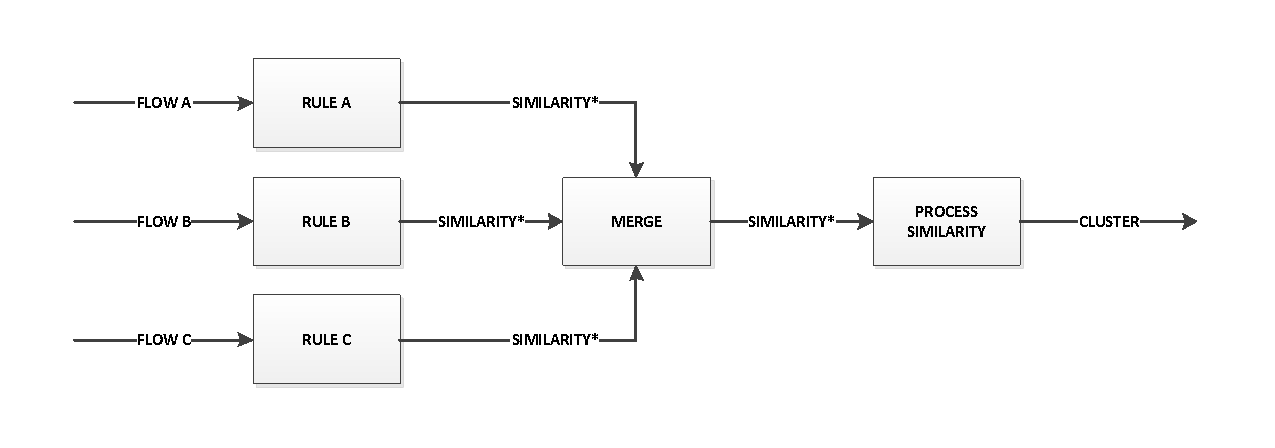
\includegraphics[width=1\textwidth]{fig/clusteringpipe}
	\caption{Clustering flow}
	\label{fig:clusteringpipe}
\end{figure}

\subsection{Assignment of e-mail addresses}
\backmatter
\end{document}
